\subsection{Результаты}
\par
Финальный результат работы алгоритма – разметка с выделением точек смены фаз и оценкой фазового состава – была представлена на рис.\ref{fig:sensor_1_final}. Так как экспертная разметка была доступна только для случая однозначной классификации каждой точки как принадлежащей одному из трех классов «вода», «нефть» или «газ», то валидацию будем проводить только для первого этапа кластеризации. 
\par
После проведения разделения датасета на три кластера по построенным признакам моделью гауссовской смеси распределений получаем разметку на рис.\ref{fig:expert_comparison}(a). На рис.\ref{fig:expert_comparison}(b). показано сравнение полученной разметки с экспертной разметкой. На экспертной разметке видно, что данные разделяются на кластеры по этим признакам не так явно, как на разметке согласно предложенному методу. 
При этом основное несовпадение приходится на «нефтяной» кластер: зеленые точки попадают в облака синих и красных точек.  Это подтверждается и матрицами ошибок, рис.\ref{fig:confusion_matrices}: согласно экспертной разметке 23\% точек «нефтяного» кластера перешли в воду, а 8\% - в газ. Результаты для остальных пяти датчиков показаны в Приложении 1.

\begin{figure}[H]
\centering
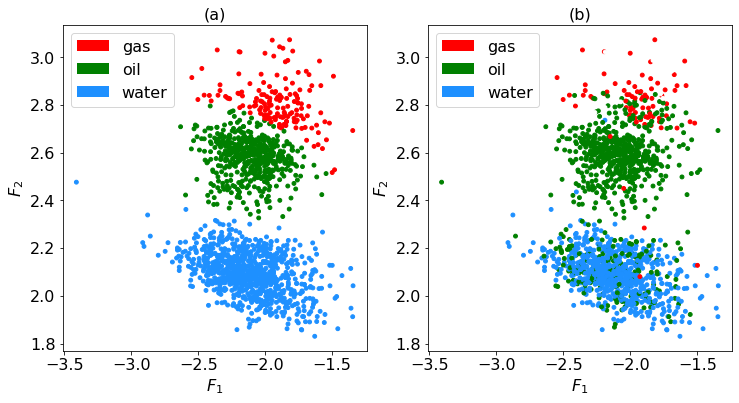
\includegraphics[width=1.0\textwidth]{TA/expert_comparison.png}
\caption{Сравнение полученной разметки (a) с экспертной (b). Синий цвет – вода, зеленый – нефть, красный – газ.}
\label{fig:expert_comparison}
\end{figure}

\begin{figure}[H]
\centering
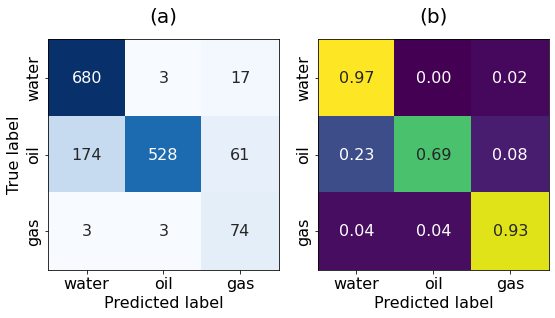
\includegraphics[width=0.6\textwidth]{TA/confusion_matrices.png}
\caption{Матрицы ошибок: (a) количество и (b) доля предсказанных значений.}
\label{fig:confusion_matrices}
\end{figure}

Одной из причин такого большого расхождения (особенно для фаз нефти и воды, которые обычно очень хорошо распознаются) является смена фаз за интервал времени цикла. В качестве примера на рис.\ref{fig:error_analysis}(d) изображен цикл, попавший в «водяной» кластер по предложенной разметке и в «нефтяной» по экспертной. Видно, что происходит смена фаз, и в начале стадии нагревания цикл действительно больше соответствует нефти, чем воде. Эти же четыре цикла показаны как точки в пространстве выбранных признаков на рис.\ref{fig:error_analysis_coordinates}.

\begin{figure}[H]
\centering
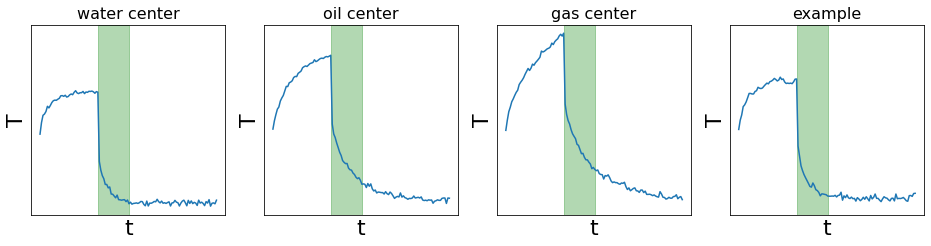
\includegraphics[width=1.0\textwidth]{TA/error_analysis.png}
\caption{Примеры циклов. Для первых трех циклов - центров кластеров - предложенная разметка совпала с экспертной. Последний цикл предложенный алгоритм определил как воду, экспертная разметка - как нефть.}
\label{fig:error_analysis}
\end{figure}

\begin{figure}[H]
\centering
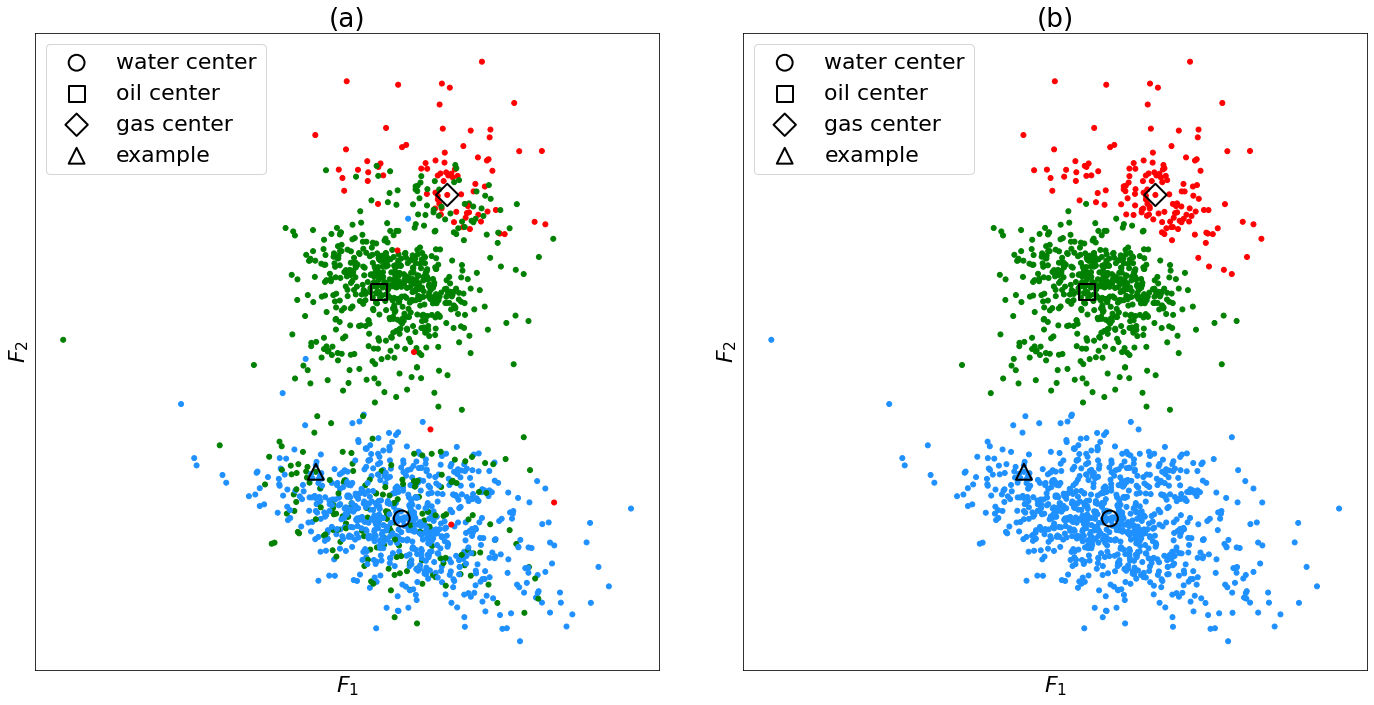
\includegraphics[width=1.0\textwidth]{TA/error_analysis_coordinates.png}
\caption{Циклы с предыдущего рисунка в пространстве выбранных координат.}
\label{fig:error_analysis_coordinates}
\end{figure}

\par
Следует отметить, что экспертная разметка проводилась на основе единственного индикатора, вычисленного на основе данных каждого цикла нагревания-охлаждения; она не является полностью ручной работой эксперта. Также без 3D-симуляции нужного уровня невозможно получить единственное решение, и в данной главе предлагается лишь еще один способ снизить неопределенность в интерпретации данных термоанемометрии. Полный цикл анализа данных должен включать в себя другие датчики и в идеале задействовать несколько различных подходов для оценки неопределенности решения; поэтому в данном случае неполное соответствие с экспертной разметкой не является проблемой.
\subsection{Обсуждение}
\par
В основе экспертной разметки, рассмотренной нами для сравнения, также лежало использование индикатора, вычисленного на основе данных каждого цикла нагревания-охлаждения (в частной беседе экспертом было указано на возможность наличия неточностей из-за неоднозначности распознавания некоторых циклов); поэтому в данном случае неполное соответствие с экспертной разметкой не является проблемой. Предложенный в данной главе новый способ нацелен на снижение неопределенности и ее оценку при интерпретации данных термоанемометрии, поскольку появляется возможность задействовать несколько различных подходов для распознавания фаз, причем в автоматическом режиме. 
\par
Оценка фазового состава должна сопровождаться и определением скоростей и массового расхода флюидов вдоль скважины. Предложенный здесь способ планируется интегрировать в эту полную задачу путем рассмотрения во взаимосвязи данных от всех шести ТА датчиков в сечении скважины, учета физики течения (например, привлечения уравнения неразрывности), траектории скважины и показаний других датчиков в сборке приборов ПГИ. Автоматизация решения этой полной задачи интерпретации на наш взгляд возможна, но потребует дальнейшего развития предложенного подхода машинного обучения без учителя. Здесь можно будет привлечь методы, разработанные в первой части работы, для выявления надежных и устойчивых индикаторов, характеризующих поток в скважине, а также учета особенностей рассматриваемых типов течений, известных из общепринятых физических моделей, полевых и лабораторных данных, опыта экспертов.